\begin{exercice*}
    Un condensateur est un composant électronique permettant de stocker de l'énergie électrique pour la restituer plus tard.
    Le graphique suivant montre l'évolution de la tension mesurée aux bornes d'un condensateur en fonction du temps lorsqu'il est en charge.
    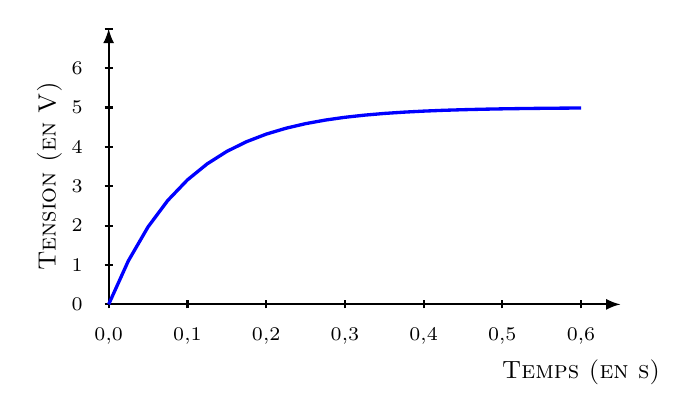
\begin{tikzpicture}[scale=1]            
        % Axes
        \draw[thick,>=latex,->](0,0)--+(6.5,0);
        \draw[thick,>=latex,->](0,0)--+(0,3.5);
        \foreach \x in {0,...,6} \draw[thick] (\x,-.05) -- (\x,0.05);
        \foreach \y in {0,...,3.5} \draw[thick] (-.05,\y) -- (0.05,\y);
        \foreach \y in {0,...,3.5} \draw[thick] (-.05,\y+0.5) -- (0.05,\y+0.5);
        \foreach \x / \label in {0/{0,0} , 1/{0,1}  , 2/{0,2}  , 3/{0,3} , 4/{0,4}  , 5/{0,5}  , 6/{0,6}} \draw (\x,-0.4) node {\scriptsize\label};
        \foreach \y / \label in {0/0, 0.5/1 , 1/2  , 1.5/3  , 2/4 , 2.5/5  , 3/6} \draw (-0.4,\y) node {\scriptsize\label};
        % Courbe
        \draw [domain=0:6,blue,very thick] plot (\x,{2.5-2.5*exp(-1*\x)});
        % LAbel axes
        \node[label={[text depth=-1ex,rotate=90]{\sc\small Tension (en V)}}] at (-0.55,1.5) {};
        \node[label={[text depth=-1ex]below:{\sc\small Temps (en s)}}] at (6,-0.45) {};			
        % Fond
        \papierMillimetre
    \end{tikzpicture}
    Justifier s'il s'agit d'une situation de proportionnalité ou non.    
\end{exercice*}
\begin{corrige}
    %\setcounter{partie}{0} % Pour s'assurer que le compteur de \partie est à zéro dans les corrigés
    %\phantom{rrr}    
    Un condensateur est un composant électronique permettant de stocker de l'énergie électrique pour la restituer plus tard.
    Le graphique suivant montre l'évolution de la tension mesurée aux bornes d'un condensateur en fonction du temps lorsqu'il est en charge.
    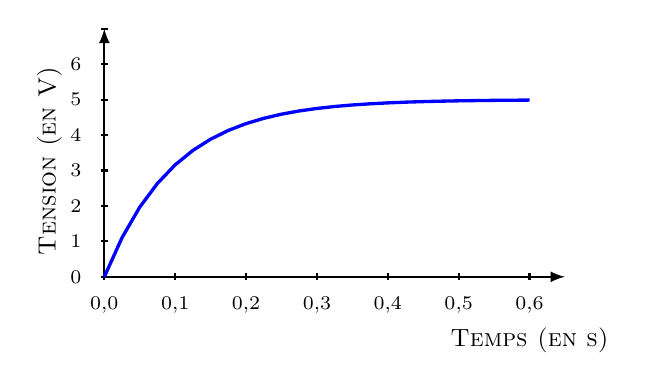
\begin{tikzpicture}[scale=0.9]            
        % Axes
        \draw[thick,>=latex,->](0,0)--+(6.5,0);
        \draw[thick,>=latex,->](0,0)--+(0,3.5);
        \foreach \x in {0,...,6} \draw[thick] (\x,-.05) -- (\x,0.05);
        \foreach \y in {0,...,3.5} \draw[thick] (-.05,\y) -- (0.05,\y);
        \foreach \y in {0,...,3.5} \draw[thick] (-.05,\y+0.5) -- (0.05,\y+0.5);
        \foreach \x / \label in {0/{0,0} , 1/{0,1}  , 2/{0,2}  , 3/{0,3} , 4/{0,4}  , 5/{0,5}  , 6/{0,6}} \draw (\x,-0.4) node {\scriptsize\label};
        \foreach \y / \label in {0/0, 0.5/1 , 1/2  , 1.5/3  , 2/4 , 2.5/5  , 3/6} \draw (-0.4,\y) node {\scriptsize\label};
        % Courbe
        \draw [domain=0:6,blue,very thick] plot (\x,{2.5-2.5*exp(-1*\x)});
        % LAbel axes
        \node[label={[text depth=-1ex,rotate=90]{\sc\small Tension (en V)}}] at (-0.55,1.5) {};
        \node[label={[text depth=-1ex]below:{\sc\small Temps (en s)}}] at (6,-0.45) {};			
        % Fond
        \papierMillimetre
    \end{tikzpicture}
    Justifier s'il s'agit d'une situation de proportionnalité ou non.\par
    \textcolor{red}{ La représentation graphique n'étant pas une droite, il ne s'agit pas d'une situation de proportionnalité.}  
\end{corrige}

